Betrachten Sie das Wavelet
\[
\psi\colon
t\mapsto
\psi(t)
=
\begin{cases}
\sin(\pi t)&\qquad -1 \le t\le 1\\
0&\qquad\text{sonst}
\end{cases}
\]
Mit diesem Wavelet soll das Signal
\[
f(t)
= 
\begin{cases}
1&\qquad 0\le t\le 1\\
0&\qquad\text{sonst}
\end{cases}
\]
analysiert werden.
\begin{teilaufgaben}
\item Rechnen Sie nach, dass $\|\psi\|=1$.
\item Überprüfen Sie, dass $\int\psi\,dt=0$.
\item Rechnen Sie nach, dass $\mathcal{W}f(-a,b)=-\mathcal{W}f(a,b)$.
Dieses Resultat erlaubt, in den folgenden Teilaufgaben nur den Fall $a>0$
zu betrachten.
\item Berechne Sie die stetige Wavelet-Transformation $\mathcal{W}f(\frac12,b)$.
\item Berechnen Sie die stetige Wavelet-Transformation $\mathcal{W}f(a,b)$
für $0<a\le\frac12$.
\item Berechne Sie die stetige Wavelet-Transformation $\mathcal{W}f(a,b)$
für $a >\frac12$.
\item Verifizieren Sie die Zulässigkeitsbedingung für das Wavelet $\psi$.
\end{teilaufgaben}

\begin{loesung}
\definecolor{pink}{rgb}{0.8,0.2,1}
\begin{figure}
%\begin{tikzpicture}[>=latex,scale=2]
%\fill[color=red!10] (0,0)--(1,0)--(1,1)--(0,1)--cycle;
%\fill[color=pink!10] plot[domain=0:180,samples=100] ({\x/180},{sin(\x)})--cycle;
%\fill[color=blue!10] plot[domain=-180:0,samples=100] ({\x/180},{sin(\x)})--cycle;
%\draw[->,line width=0.7pt] (-3.1,0)--(3.3,0) coordinate[label={$t$}];
%\draw[->,line width=0.7pt] (0,-1.1)--(0,1.3) coordinate[label={right:$f(t)$}];
%\draw[line width=1pt,color=red] (-3,0)--(0,0);
%\draw[line width=0.3pt,color=red] (0,0)--(0,1);
%\draw[line width=1pt,color=red] (0,1)--(1,1);
%\draw[line width=0.3pt,color=red] (1,0)--(1,1);
%\draw[line width=1pt,color=red] (1,0)--(3,0);
%
%\draw[color=blue,line width=1pt] (-3,0)--
%	plot[domain=-180:180,samples=100] ({\x/180},{sin(\x)})
%	--(3,0);
%\end{tikzpicture}
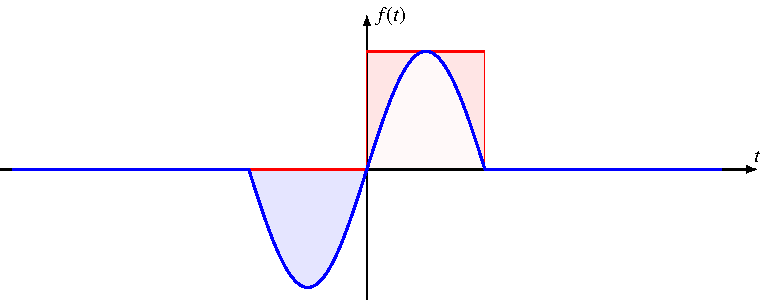
\includegraphics{chapters/uebungsaufgaben/04001-signal.pdf}
\caption{Signal $f(t)$ (rot) und Wavelet $\psi$ (blau) für Aufgabe~4.1.
\label{04001:funktionen}}
\end{figure}
Eine graphische Darstellung der Funktionen $f$ und $\psi$ ist in
Abbildung~\ref{04001:funktionen} zu finden.
\begin{teilaufgaben}
%
% Loesung Teilaufgabe a)
%
\item
Beweis durch Nachrechnen:
\begin{align*}
\|\psi\|^2
&=
\int_{-\infty}^\infty |\psi(t)|^2\,dt
=
\int_{-1}^1 \sin^2(\pi t)\,dt
=
\int_{-1}^1 \frac{1-\cos 2\pi t}{2}\,dt
\\
&=
\frac12\biggl[
t-\frac{1}{2\pi}\sin 2\pi t
\biggr]_{-1}^{1}
=\frac12(1-(-1))
=
1.
\end{align*}
Alternativ kann man aus Symmetriebetrachtungen erkennen, dass der Graph
von $\psi(t)^2$ das Rechteck mit Ecken $(-1,0)$ und $(1,1)$ halbiert.
Da das Rechteck den Flächeninhalt $2$ hat, folgt die Normierungsbedingung.
%
% Lösung Teilaufgabe b)
%
\item
Das Wavelet $\psi$ ist eine ungerade Funktion, daher verschwindet ihr
Integral.
%
% Lösung Teilaufgabe c)
%
\item
Für das Wavelet gilt $\psi(-t)=-\psi(t)$.
\begin{align*}
\mathcal{W}f(-a,b)
&=
\int_{-\infty}^\infty f(t)\psi((t-b)/(-a))\,dt
=
-\int_{-\infty}^\infty f(t)\psi((t-b)/a)\,dt
=
-\mathcal{W}f(a,b).
\end{align*}
%
%
%
\item
In diesem Fall ist das Wavelet
\[
\psi_{a,b}(t)
=
\psi_{\frac12,b}(t)
=
\begin{cases}
\sqrt{2}\sin 2\pi t&\qquad b-\frac12\le t\le b+\frac12
\\
0&\qquad\text{sonst.}
\end{cases}
\]
Es hat daher als Träger genau das Interval $[b-\frac12,b+\frac12]$.
Dies bedeutet, dass wir vier Fälle unterscheiden müssen:
\begin{enumerate}
\item
Fall $b < -\frac12$:  Der Träger von $\psi_{a,b}$ liegt ausserhalb des
intervals $[0,1]$, das Skalarprodukt
$\langle f,\psi_{a,b}\rangle=\mathcal{W}f(a,b)=0$ verschwindet.
\item
Fall $-\frac12\le b < 0$: In diesem Fall liegt das linke Ende des Trägers
von $\psi_{a,b}$ ausserhalb des Intervals $[0,1]$, das Integral zur Berechnung
von $\mathcal{W}f(a,b)$ ist also nur von $0$ bis $b+\frac12$ zu erstrecken:
\begin{align*}
\mathcal{W}f({\textstyle\frac12},b)
&=
\int_{0}^{b+\frac12} \sqrt{2} \sin 2\pi(t-b)\,dt
=
\biggl[
-
\frac{\sqrt{2}}{2\pi}
\cos 2\pi(t-b)
\biggr]_0^{b+\frac12}
\\
&=
-\frac{\sqrt{2}}{2\pi}(\cos\pi - \cos(2\pi b))
=
\frac{\sqrt{2}}{2\pi}(1+\cos(2\pi b))
=
\frac{\sqrt{2}}{\pi}
\cos^2 \pi b.
\end{align*}
\item
Fall $0\le b \le \frac12$: In diesem Fall ist das Integral nur von $b-\frac12$
zu $1$ zu erstrecken:
\begin{align*}
\mathcal{W}f({\textstyle\frac12},b)
&=
\int_{b-\frac12}^1 \cos 2\pi (t-b)\,dt
=
\biggl[
-\frac{\sqrt{2}}{2\pi}\cos 2\pi(t-b)
\biggr]_0^{b-\frac12}
\\
&=
-\frac{\sqrt{2}}{2\pi}(
\cos 2\pi(1-b)
-
\cos \pi
)
=
-\frac{\sqrt{2}}{2\pi}(1+\cos 2\pi(1-b))
\\
&=
-\frac{\sqrt{2}}{\pi}\cos^2\pi(1-b).
\end{align*}
\item
Fall $b > \frac12$:
Wie im ersten Fall verschwindet die Wavelet-Transformation auch in diesem
Fall.
\end{enumerate}
Der Graph von $b\mapsto \mathcal{W}f(\frac12,b)$ ist in
Abbildung~\ref{04001:wavelet2} dargestellt.
\begin{figure}
\centering
%\begin{tikzpicture}[>=latex,scale=4]
%\def\vs{1}
%
%\foreach \a in {0.25,0.125,0.0625}{
%\draw[color=red!40,line width=1pt]
%	(-1.1,0)--({-\a},0)--
%	plot[domain={-\a}:{\a},samples=100]
%		({\x},{\vs*\a*(1+cos((\x/\a)*180))/(sqrt(\a)*3.1415)})
%	--
%	plot[domain={1-\a}:{1+\a},samples=100]
%		({\x},{-\vs*\a*(1+cos(((1-\x)/\a)*180))/(sqrt(\a)*3.1415)})
%	--(2.05,0);
%}
%\draw[->,line width=0.7pt] (-1.1,0)--(2.1,0)
%	coordinate[label={$b$}];
%\draw[->,line width=0.7pt] (0,-0.6)--(0,0.6)
%	coordinate[label={right:$\mathcal{W}f(a,b)$}];
%\def\a{0.5}
%\draw[color=red,line width=1pt] (-1.1,0)--(-0.5,0)--
%	(-1.1,0)--({-\a},0)--
%	plot[domain={-\a}:{\a},samples=100]
%		({\x},{\vs*\a*(1+cos((\x/\a)*180))/(sqrt(\a)*3.1415)})
%	--
%	plot[domain={1-\a}:{1+\a},samples=100]
%		({\x},{-\vs*\a*(1+cos(((1-\x)/\a)*180))/(sqrt(\a)*3.1415)})
%	--(2.05,0);
%
%\draw[line width=0.7pt] (-1,-0.025)--(-1,0.025);
%\draw[line width=0.7pt] (1,-0.025)--(1,0.025);
%\draw[line width=0.7pt] (2,-0.025)--(2,0.025);
%\node at (-1,-0.025) [below] {$-1$};
%\node at (1,-0.025) [below] {$1$};
%\node at (2,-0.025) [below] {$2$};
%\end{tikzpicture}
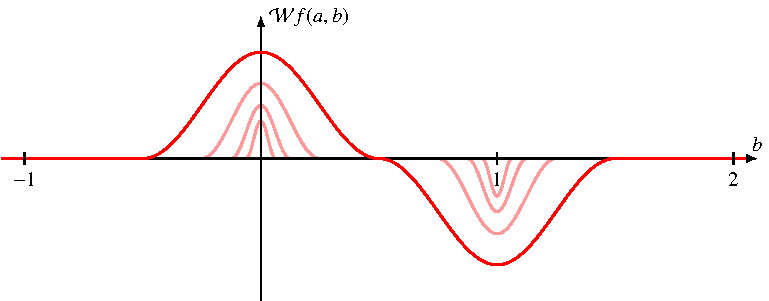
\includegraphics{chapters/uebungsaufgaben/04001-W.pdf}
\caption{Werte der stetige Wavelet-Transformation $\mathcal{W}f(\frac12,b)$
(rot)
für das Signal $f$ und das Signal $\psi$ aus Abbildung~\ref{04001:funktionen}.
Die Werte der Wavelet-Transformation $\mathcal{W}f(a,b)$ für
$a=\frac14,\frac18,\frac1{16}$ sind hellrot gezeichnet.
Die Wavelet-Transformation detektiert die Sprungstellen bei $t=0$ und
$t=1$, die Genauigkeit steigt je kleiner $a$ ist.
\label{04001:wavelet2}}
\end{figure}
%
% Lösung von Teilaufgabe d)
%
\item
Für $a\le\frac12$ wird das Wavelet von der $D_a$-Operation so stark gestaucht,
dass höchstens ein Endpunkt des Intervals $[0,1]$ im Träger der Funktion
$\psi_{a,b}$ liegen kann.
Der Träger des Wavelets liegt jetzt im Interval $[b-a,b+a]$.
Es gibt nun aber fünf Fälle zu berücksichtigen
\begin{enumerate}
\item Fall $b\le -a$:
Die Träger von $\psi_{a,b}$ und $f$ schneiden
sich nicht, $\mathcal{W}f(a,b)=0$.
\item Fall $-a\le b \le a$:
Wie im Fall $a=\frac12$ berechnet man
\begin{align*}
\mathcal{W}f(a,b)
&=
\int_{0}^{b+a} \frac{1}{\sqrt{|a|}} \sin \pi(t-b)/a\,dt
=
\biggl[
-
\frac{a}{\pi\sqrt{|a|}}
\cos \pi(t-b)/a
\biggr]_0^{b+a}
\\
&=
-\frac{a}{\pi\sqrt{|a|}}(\cos\pi - \cos\pi \frac{b}{a}))
=
\frac{a}{\pi\sqrt{|a|}}(1+\cos(\pi \frac{b}{a}))
\\
&=
\frac{a}{2\pi\sqrt{|a|}}\cos^2\frac{\pi b}{2a}.
\end{align*}
\item Fall $a\le b \le 1-a$:
Der Träger von $\psi_{a,b}$ liegt ganz innerhalb des Intervals $[0,1]$,
es wird also $\psi_{a,b}$ über den ganzen Träger integriert.
Dieses Integral verschwindet, also 
$\mathcal{W}f(a,b)=0$.
\item Fall $1-a\le b \le 1 +a$:
Wie im Fall $a=\frac12$ berechnet man
\begin{align*}
\mathcal{W}f(a,b)
&=
\int_{b-a}^{1} \frac{1}{\sqrt{|a|}} \sin \pi\frac{t-b}{a}\,dt
=
\biggl[
-
\frac{a}{\pi\sqrt{|a|}}
\cos \pi\frac{t-b}{a}
\biggr]_{b-a}^1
\\
&=
-\frac{a}{\pi\sqrt{|a|}}(
\cos\pi \frac{1-b}{a}
-
\cos\pi 
)
=
-\frac{a}{\pi\sqrt{|a|}}\biggl(1+\cos\pi\frac{1- b}{a}\biggr)
\\
&=
-\frac{a}{2\pi\sqrt{|a|}}\cos^2\frac{\pi(1- b)}{2a}.
\end{align*}
\item Fall $1+a\le b$:
Die Träger von $\psi_{a,b}$ und $f$ schneiden
sich nicht, $\mathcal{W}f(a,b)=0$.
\end{enumerate}
%
% Lösung von Teilaufgabe e), a > 1/2
%
\item
Der Träger der Funktion $\psi_{a,b}(t)$ ist das Interval $[b-a,b+a]$.
Die folgenden Fälle sind zu unterscheiden
\begin{enumerate}
\item
Fall $b+a < 0$: die Träger von $\psi_{a,b}$ und von $f$ sind disjunkt,
daher ist $\mathcal{W}f(a,b)=0$ in diesem Fall.
\item 
Fall $0\le b+a\le 1$: das Integral ist über das Interval von $0$ bis $a+b$ zu
erstrecken:
\begin{align*}
\mathcal{W}f(a,b)
&=
\frac{1}{\sqrt{|a|}}
\int_0^{b+a} \sin\pi\frac{t-b}{a}\,dt
=
\frac{1}{\sqrt{|a|}}
\biggl[
-\frac{a}{\pi} \cos\frac{t-b}{a}
\biggr]_0^{b+a}
\\
&=
-
\frac{1}{\sqrt{|a|}}
\frac{a}{\pi}
\biggl(
\cos \pi
-
\cos\frac{\pi b}{a}
\biggr)
=
\frac{a}{\pi\sqrt{|a|}}
\biggl(1+\cos\frac{\pi b}{a}\biggr).
\end{align*}
\item
Fall $b-a \le 0$ und $1 \le b+a$: In diesem Fall ist der Träger von $f$
ganz im Träger von $\psi_{a,b}$ enthalten, das Integral ist also über das
Interval $[0,1]$ zu erstrecken:
\begin{align*}
\mathcal{W}f(a,b)
&=
\frac{1}{\sqrt{|a|}}
\int_0^1 
\sin \pi\frac{t-b}{a}
\,dt
=
\frac{1}{\sqrt{|a|}}
\biggl[
-\frac{a}{\pi} \cos\frac{t-b}{a}
\biggr]_0^1
\\
&=
-\frac{1}{\sqrt{|a|}}
\frac{a}{\pi}
\biggl(
\cos\pi\frac{1-b}{a}
-
\cos\pi \frac{b}{a}
\biggr).
\end{align*}
\item
Fall $0\le b-a\le 1$: Das Integral ist zu erstrecken über das Interval
$[b-a,1]$:
\begin{align*}
\mathcal{W}f(a,b)
&=
\frac{1}{\sqrt{|a|}}
\int_{b-a}^1
\sin\pi\frac{t-b}{a}\,dt
=
\frac{1}{\sqrt{|a|}}
\biggl[
-
\frac{a}{\pi} \cos\pi\frac{t-b}{a}
\biggr]_{b-a}^1
\\
&=
-
\frac{1}{\sqrt{|a|}}
\frac{a}{\pi}
\biggl(
\cos\pi
-
\cos\pi\frac{1-b}{a}
\biggr)
=
\frac{1}{\sqrt{|a|}}
\frac{a}{\pi}\biggl(
1+\cos\pi\frac{1-b}a
\biggr).
\end{align*}
\item
Fall $1<b-a$: die Träger von $\psi_{a,b}$ and $f$ schneiden sich nicht,
also ist $\mathcal{W}f(a,b)=0$.
\end{enumerate}
%
% Lösung von Teilaufgabe f) Zulässigkeitsbedingung
%
\begin{figure}
\centering
%\begin{tikzpicture}[>=latex]
%\def\perioden{5}
%\draw[->,line width=0.7pt] (-6.3,0)--(6.5,0) coordinate[label={$\omega$}];
%\draw[->,line width=0.7pt] (0,-0.8)--(0,2.5) coordinate[label={right:$\operatorname{Im}\hat{\psi}(\omega)|$}];
%\draw[color=red,line width=1pt] plot[domain=-{\perioden*360+1}:{\perioden*360+1},samples=300]
%	({\x*3.1415/(\perioden*180)},{5*(sqrt(2)/sqrt(3.14159))*sin(\x)*(\x/180)/(3.14159*(1-(\x/180)*(\x/180)))});
%\foreach \x in {-10,...,10}{
%	\draw[line width=0.7pt] ({\x*3.1415/\perioden},-0.1)--({\x*3.1415/\perioden},0.1);
%	\node at ({3.14159/\perioden},-0.1) [below] {$\pi$};
%	\node at ({-3.14159/\perioden},-0.1) [below] {$-\pi$};
%}
%\end{tikzpicture}
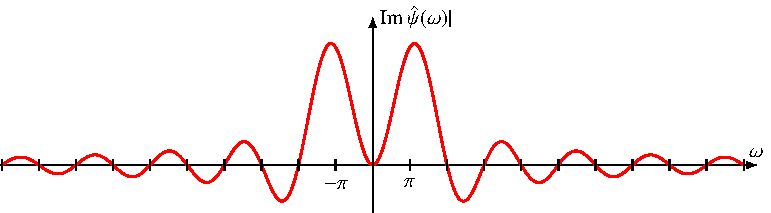
\includegraphics{chapters/uebungsaufgaben/04001-spektrum.pdf}
\caption{Fourier-Spektrum des Wavelets von Aufgabe~\ref{04001}.
\label{04001:spektrum}}
\end{figure}
\item
Zwar folgt die Zulässigkeitsbedingung für $\psi$ aus dem
Satz~\ref{satz:zulaessigkeit} und der in Teilaufgabe b) bewiesenen
Tatsache, dass $\int \psi(t)\,dt=0$, doch können wir sie in diesem Fall
auch direkt nachweisen.
Dazu berechnen wir zunächst die Fourier-Transformierte des Wavelets:
\begin{align}
\hat{\psi}(\omega)
&=
\frac{1}{\sqrt{2\pi}}
\int_{-\infty}^\infty \psi(t)e^{-i\omega t}\,dt
=
\frac{1}{\sqrt{2\pi}}
\int_{-1}^{1} \sin(\pi t)e^{-i\omega t}\,dt
=
\frac{1}{\sqrt{2\pi}}
\int_{-1}^1
\frac1{2i} (e^{i\pi t}-e^{-i\pi t})e^{-i\omega t}\,dt.
\label{04001:fourier1}
\end{align}
Darin haben wir die komplexe Darstellung der Sinus-Funktion verwendet.
Die Integrale über die komplexen Exponentialfunktionen können explizit
ausgewertet werden:
\begin{align*}
\int_{-1}^1 \frac{1}{2i}e^{i(\pi-\omega)t}\,dt
&=
\biggl[
\frac{1}{i(\pi-\omega)}
\frac1{2i}
e^{i(\pi-\omega)t}
\biggr]_{-1}^1
=
\frac{1}{i(\pi-\omega)}
\cdot
\frac1{2i}(e^{i(\pi-\omega)}-e^{-i(\pi-\omega)})
\\
&=
\frac{\sin(\pi-\omega)}{i(\pi-\omega)}
=
-i\frac{\sin(\omega)}{\pi-\omega}
\\
\int_{-1}^1 \frac{1}{2i}e^{-i(\pi+\omega)t}\,dt
&=
\biggl[
-\frac{1}{i(\pi+\omega)}
\frac1{2i}
e^{-i(\pi+\omega)t}
\biggr]_{-1}^1
=
-\frac{1}{i(\pi+\omega)}
\cdot
\frac1{2i}(e^{-i(\pi+\omega)}-e^{i(\pi+\omega)})
\\
&=
\frac{\sin(\pi+\omega)}{i(\pi+\omega)}
=
i\frac{\sin(\omega)}{\pi+\omega}.
\end{align*}
Zusammen mit \eqref{04001:fourier1} finden wir jetzt für die
Fourier-Transformation
\begin{align}
\hat{\psi}(\omega)
&=
\frac{1}{\sqrt{2\pi}}
\biggl(
\frac{\sin(\pi-\omega)}{i(\pi-\omega)}
-
\frac{\sin(\pi+\omega)}{i(\pi+\omega)}
\biggr)
=
\frac{i\sin\omega}{\sqrt{2\pi}}
\frac{\pi+\omega-\pi+\omega}{\pi^2-\omega^2}
=
\frac{i\sin\omega}{\sqrt{2\pi}}
\frac{2\omega}{\pi^2-\omega^2}.
\label{04001:fourier2}
\end{align}
Wegen 
\[
\lim_{x\to 0}\frac{\sin x}{x}
\]
kann man am ersten Ausdruck von \eqref{04001:fourier2} ablesen,
dass $\hat{\psi}$ beschränkt ist trotz der Nullstellen der Nenner
bei $\pm \pi$.
Für $\omega\to\infty$ fällt $\hat{\psi}$ wie $1/|\omega|$, somit fällt
$|\hat{\psi}(\omega)|^2/|\omega|$ wie $1/|\omega|^3$, was sicher
integrierbar ist.
Es ist also nur noch zu klären, ob auch das Integral bei $\omega=0$
konvergiert.
Aus der letzten Form in~\eqref{04001:fourier2} folgt, dass
\[
\lim_{\omega\to\infty} \frac{|\hat{\psi}(\omega)|^2}{|\omega|}
=
\frac{2}{\pi}
\lim_{\omega\to\infty} \frac{|\omega|}{\pi^2-\omega^2}\sin^2\omega
=
0.
\]
Die Funktion $|\hat{\psi}(\omega)|^2/|\omega|$ ist daher in einer
Umgebung von $0$ beschränkt und stetig.
Wir können daher schliessen, dass
\[
\int_{\infty}^\infty\frac{|\hat{\psi}(\omega)|^2}{\omega}\,d\omega < \infty,
\]
das Wavelet $\psi$ erfüllt die Zulässigkeitsbedingung.
\qedhere
\end{teilaufgaben}
\end{loesung}
